\documentclass[a4paper, 11pt]{article}
\usepackage{geometry}
\usepackage{indentfirst}
\usepackage{setspace}
\usepackage{amsmath}
\usepackage{graphicx}
\usepackage{wrapfig}
\usepackage{caption}
\usepackage{indentfirst}
\setlength{\parindent}{20pt}
\usepackage{amssymb}
\usepackage{float}
\usepackage{subcaption}

\graphicspath{ {./images/} }
\geometry{left=2.5cm, right=2.5cm, top=2.5cm, bottom=2.5cm}

\begin{document}	
	\title{Exercise \# 3. Numerical Solution of the Poisson Problem. }
	\author{{\small Alexandre Rodrigues (2039952)}}
	\date{\today}
	
	\maketitle
		\section{Method}
			I will describe relevant steps of developing this implementation and respective theory.
			
			1- input files from specified mesh
			
			2- create pattern for the stifness matrix
			...
			
			3- local stifness matrix
			
		
		
		\section{Results}
		
			\subsection*{Level 0}
				\begin{figure}[H]
					\begin{subfigure}{.49\textwidth}
						\centering
						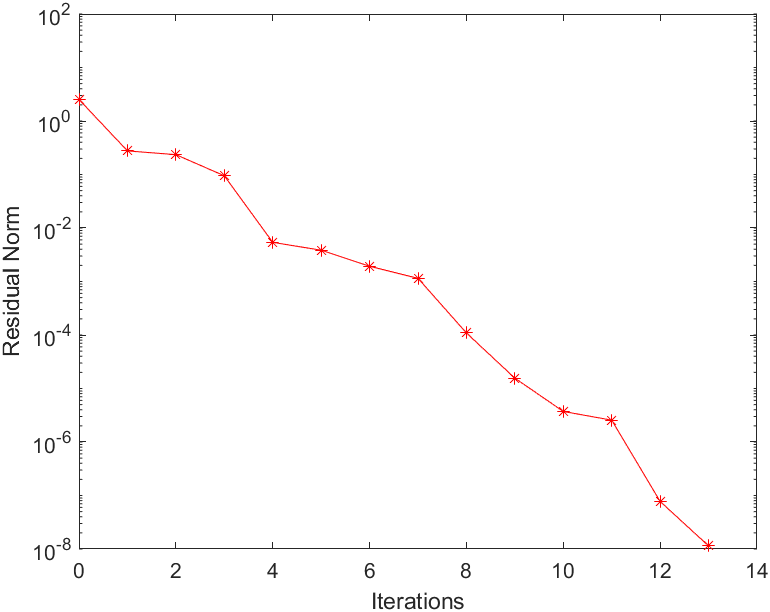
\includegraphics[width=.99\linewidth]{img0/J.png}  
						\caption{Jacobi}
						\label{fig:Jacobi_0}
					\end{subfigure}
					\begin{subfigure}{.49\textwidth}
						\centering
						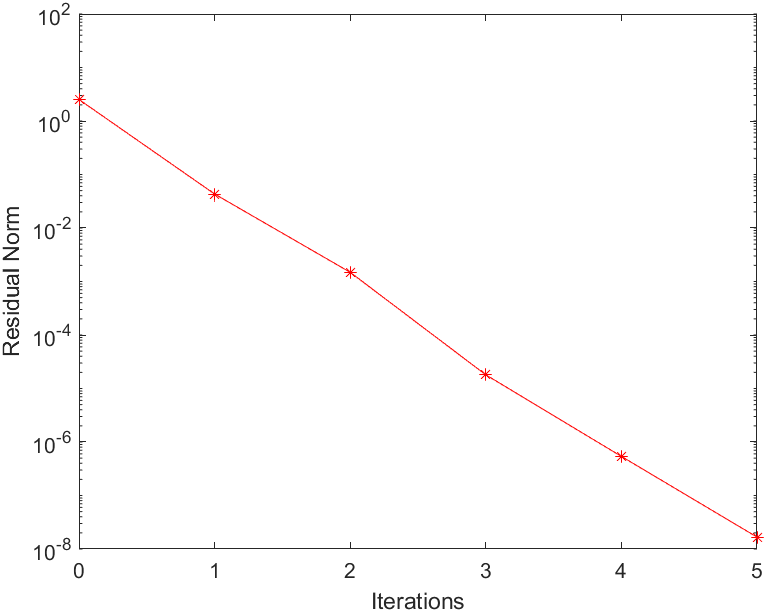
\includegraphics[width=.99\linewidth]{img0/C.png}  
						\caption{Choledsky}
						\label{fig:Chol_0}
					\end{subfigure}
					\caption{Convergence plots for level 0}
					\label{fig:fig0}
				\end{figure}
				
			
			\subsection*{Level 1}
				\begin{figure}[H]
					\begin{subfigure}{.49\textwidth}
						\centering
						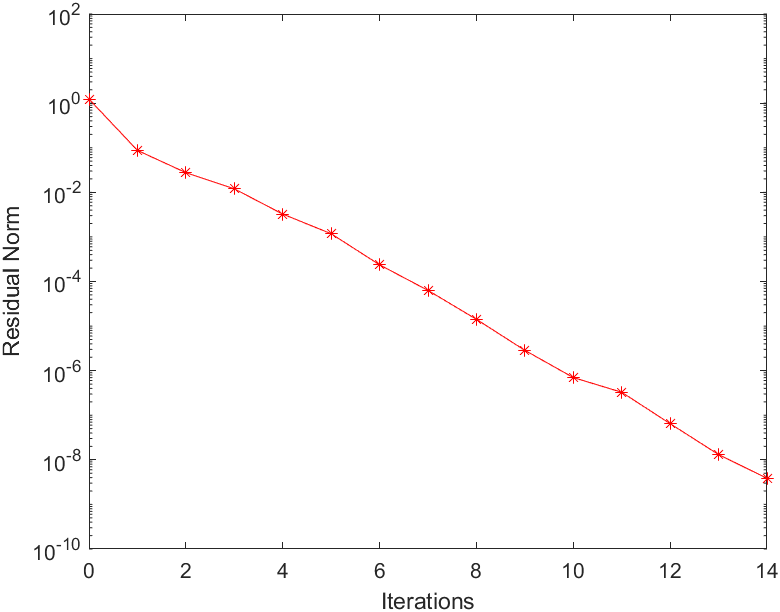
\includegraphics[width=.99\linewidth]{img1/J.png}  
						\caption{Jacobi}
						\label{fig:Jacobi_1}
					\end{subfigure}
					\begin{subfigure}{.49\textwidth}
						\centering
						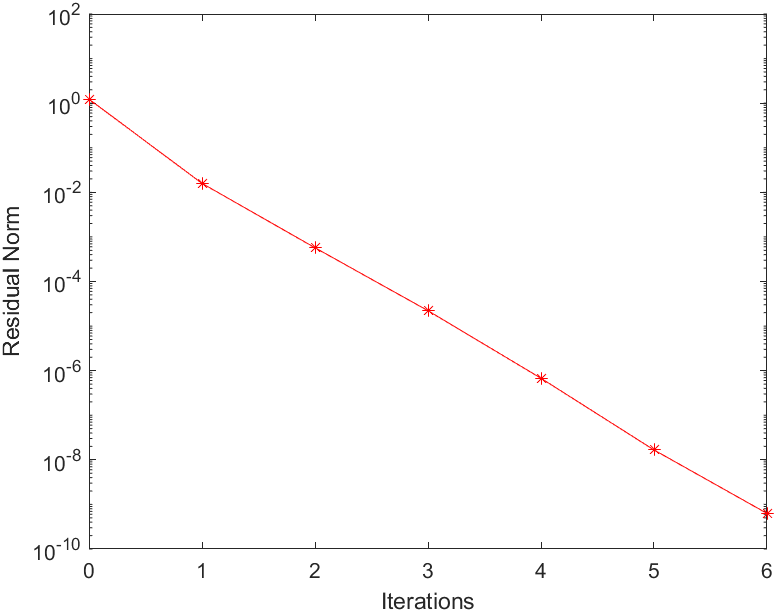
\includegraphics[width=.99\linewidth]{img1/C.png}  
						\caption{Choledsky}
						\label{fig:Chol_1}
					\end{subfigure}
					\caption{Convergence plots for level 1}
					\label{fig:fig1}
				\end{figure}
			
			\subsection*{Level 2}
				\begin{figure}[H]
					\begin{subfigure}{.49\textwidth}
						\centering
						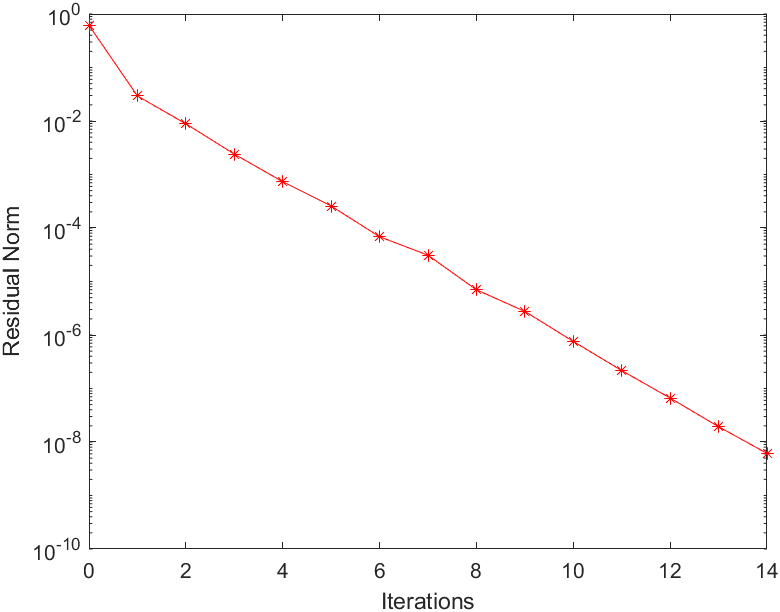
\includegraphics[width=.99\linewidth]{img2/J.png}  
						\caption{Jacobi}
						\label{fig:Jacobi_2}
					\end{subfigure}
					\begin{subfigure}{.49\textwidth}
						\centering
						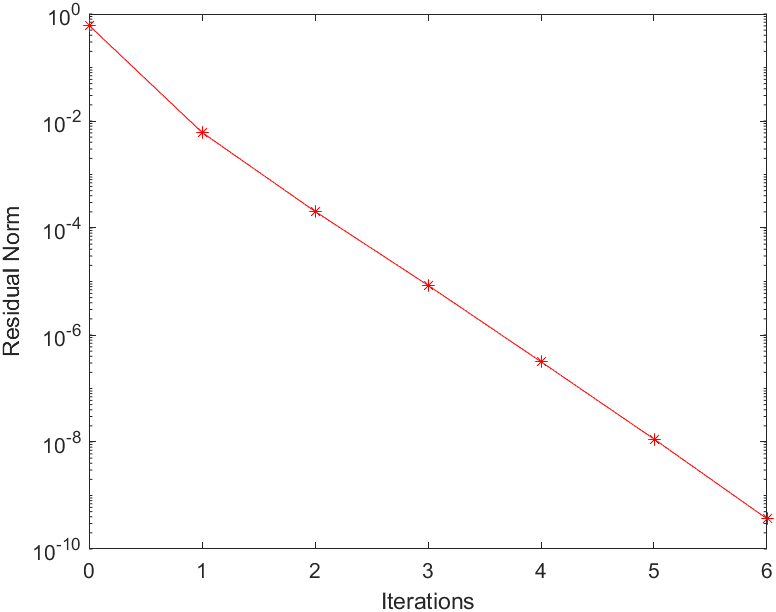
\includegraphics[width=.99\linewidth]{img2/C.png}  
						\caption{Choledsky}
						\label{fig:Chol_2}
					\end{subfigure}
					\caption{Convergence plots for level 2}
					\label{fig:fig2}
				\end{figure}
			
			\subsection*{Level 3}
				\begin{figure}[H]
					\begin{subfigure}{.49\textwidth}
						\centering
						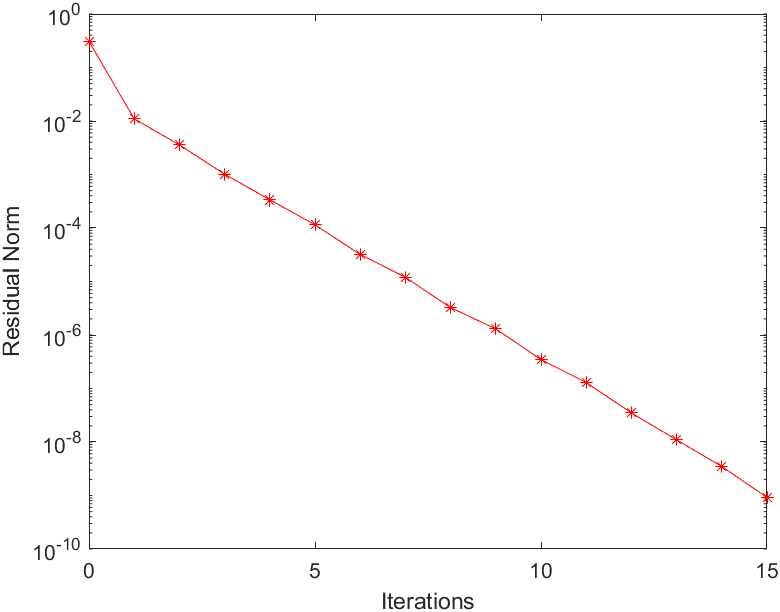
\includegraphics[width=.99\linewidth]{img3/J.png}  
						\caption{Jacobi}
						\label{fig:Jacobi_3}
					\end{subfigure}
					\begin{subfigure}{.49\textwidth}
						\centering
						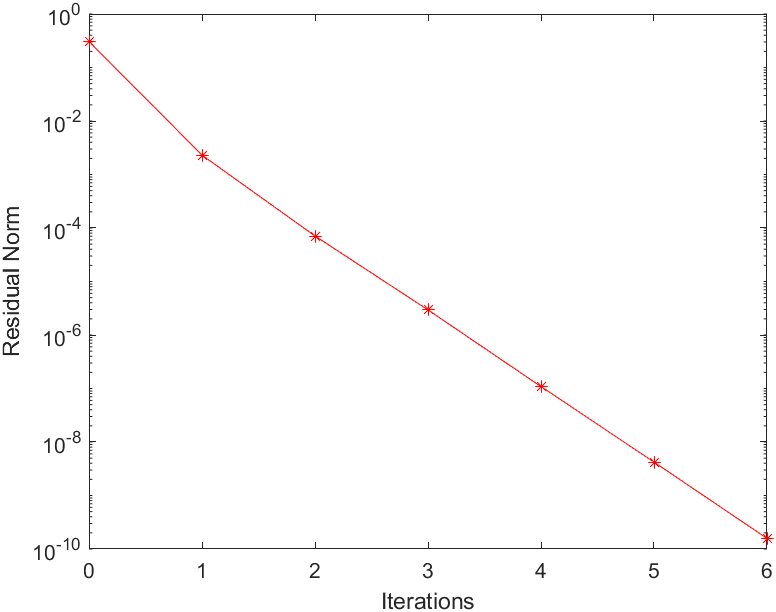
\includegraphics[width=.99\linewidth]{img3/C.png}  
						\caption{Choledsky}
						\label{fig:Chol_3}
					\end{subfigure}
					\caption{Convergence plots for level 3}
					\label{fig:fig3}
				\end{figure}
			
			\subsection*{Level 4}
				\begin{figure}[H]
					\begin{subfigure}{.49\textwidth}
						\centering
						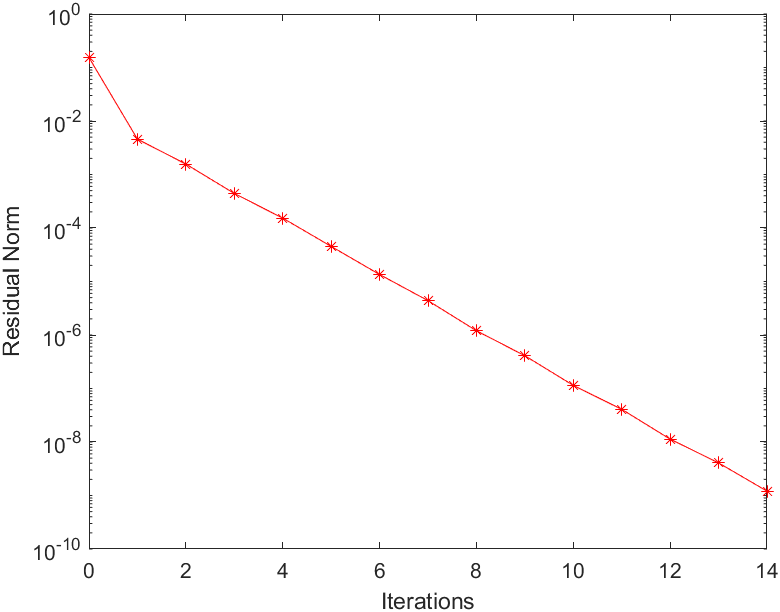
\includegraphics[width=.99\linewidth]{img4/J.png}  
						\caption{Jacobi}
						\label{fig:Jacobi_4}
					\end{subfigure}
					\begin{subfigure}{.49\textwidth}
						\centering
						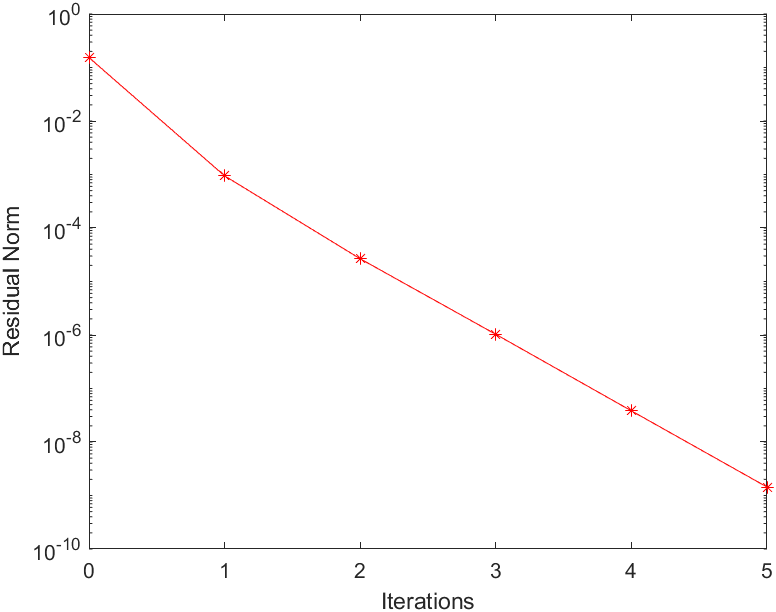
\includegraphics[width=.99\linewidth]{img4/C.png}  
						\caption{Choledsky}
						\label{fig:Chol_4}
					\end{subfigure}
					\caption{Convergence plots for level 4}
					\label{fig:fig4}
				\end{figure}
			
			\subsection{Epsilon}
				\begin{table}[H]
					\centering
%					\begin{tabular}{c|c|c}
%						\textbf{Level} 	& \textbf{$ \epsilon $} & \textbf{ Error Ratio}  \\ \hline
%						$ 0  $			& $ 0.9931 $ & N/A \\ \hline
%						$ 1  $			& $ 1.0231 $ & $ 1.0302 $ \\ \hline
%						$ 2  $			& $ 1.0217 $ & $ 0.9986 $ \\ \hline
%						$ 3  $			& $ 1.0190 $ & $ 0.9974 $ \\ \hline
%						$ 4  $			& $ 1.0176 $ & $ 0.9986 $ \\ 
%					\end{tabular}
					\begin{tabular}{c|c|c}
						\textbf{Level} 	& \textbf{$ \epsilon $} & \textbf{ Error Ratio}  \\ \hline
						$ 0  $			& $ 0.9931 $ 			& N/A \\ \hline
						$ 1  $			& $ 1.0508 $ 			& $ 1.0581 $ \\ \hline
						$ 2  $			& $ 1.0629 $ 			& $ 1.0115 $ \\ \hline
						$ 3  $			& $ 1.0657 $	 		& $ 1.0026 $ \\ \hline
						$ 4  $			& $ 1.0664 $ 			& $ 1.0007 $ \\ 
					\end{tabular}
					\caption{FEM Convergence table}
					\label{table:errors}
				\end{table}
				The $ \epsilon $ value slightly increases on each step of refinement....??
	
	
\end{document}



